\chapter{Conclusion}

\minitoc

This chapter will describe the final version of our product and what we have found during this project. Also we will discuss the further development of the system and what improvement can be made.

\clearpage

\section{Final Product}
The system we have created is a basic library system, and it allows users to store information on books and authors. It is a web application, meaning it is accessed through a web- browser. It separates itself from regular web- applications in that it incorporates a console. The system consists of two main components, a client part and a server with an associated database. The client part deals with user input while the server provides the clients the ability to persistently store data between user sessions. 

\subsubsection{Client}
A screenshot of the client is shown in Figure~\ref{figure:wonsoleScreenshot}. The client part of the system is implemented using web technologies like JavaScript, jQuery, HTML and CSS. The interface is split in two separate views, one containing the console, and one containing a simple GUI for the application. The GUI part consists of two views, showing either a list of objects, or specifics on one single object. This part of the application offers limited functionality, which is confined to navigation of the application and editing of existing objects.

\begin{figure}[H]
\centering
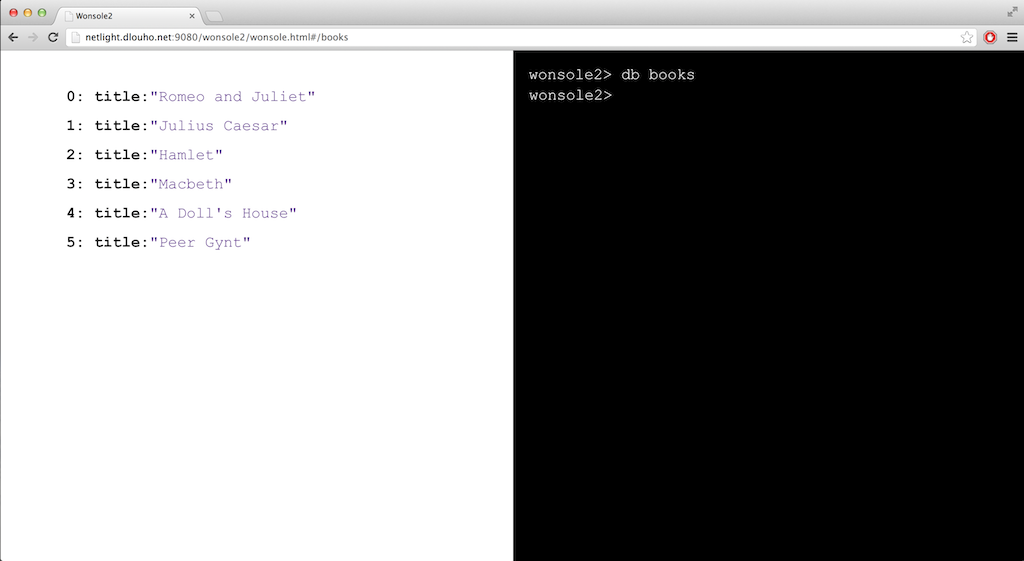
\includegraphics[width=5in]{image/wonsoleScreenshot.png}
\caption{Client Screenshot}
\label{figure:wonsoleScreenshot}
\end{figure}

The console on the other hand contains a rich set of functionality. The main purpose of the console is to expose the underlying objects of the system, and it allows for the user to modify the properties of these objects. It comes with a list of predefined commands that represents commonly used actions such as add, delete and navigation between the different databases. The commands offers a layer of abstraction to the users, and makes it easier for inexperienced users to utilise the console. The commands are functions written in JavaScript, and when recognised by the console/parser the console makes a call to these functions. The console is also capable of running any JavaScript code, meaning anything that is not recognised as a command is executed as regular JavaScript in the browser. This gives the user the ability to define their own functions, and extend the functionality of the console.

\subsubsection{Server}
The database of the system is implemented using CouchDB, which functions as a standalone server system. The CouchDB consists of a set of databases, each holding a group of objects with their associated attributes. Our system contains two databases, one for book objects and one for author objects. The communication between client and server is done through a RESTful api that CouchDB creates automatically. This api contains a rich set of functionality, and allows for actions such as add, delete, update and filter. 

\section{Chosen Technologies}
We spent a lot of time on the pre- study and on research in this project, and we feel it was well worth the effort. Also our customer helped us a lot, and offered great suggestions and guidance throughout the project. The technologies we ended up using were not only new and exciting, but were also a great fit together. JavaScript, jQuery, JSON, HTML and CSS are robust and mature web technologies in use all over the world today. Coupled with CouchDB, which was designed from the ground with web- applications in mind, they make a powerful collection of technologies that work well together.

Probably the most important decision on technology we were left with after the pre- study was whether to go for a traditional database management system like MySQL, or choose a more unconventional NoSQL system. The customer did not specify any requirements concerning the performance or stability of the server in this project, and indicated that the specifics on the server implementation was not that important to them. As a result we wanted it to be as simple as possible. After a detailed look at the needs for this project we ended up choosing a NoSQL database in the form of CouchDB. The reason for this was that CouchDB provided us with many advantages that a traditional relational database could not. Our system is heavily centered around JavaScript objects and their attributes. CouchDB, and other document oriented NoSQL systems, stores data in the form of objects directly in JSON format, which is a simple textual notation for JavaScript objects. This implied a minimal amount of work getting the client and server to communicate. If we had opted to use a traditional SQL system for the database we would have needed more extensive server side technologies, like PHP or ASP.NET to handle the database and to do database-object parsing. All of this was avoided by choosing CouchDB, which is able to work without any extra server software, and automatically creates a RESTful api to interact with the database. 

Whereas trying to add undefined attributes to an existing record in a traditional relational database management system would result in an error, CouchDB automatically adds these attributes to the stored object. In essence, it allows us to add any new attribute to the existing objects, as long as it's represented in JSON format. This obviously gives you great flexibility. To do something similar in a regular SQL system you would have to change the schema of the database table every time a new attribute was discovered, or be able to model every aspect of the objects from the beginning. For non-trivial real world domains, this usually presents a difficult challenge. Also the job of representing complex objects are considerably less than in a relational database. Complex object representation in SQL often requires a tedious process to identify the different tables you need and the relations between them. In CouchDB this job is reduced to just putting the entire JavaScript object directly into the database, which saves a lot of time for the developer. Maybe the best experience from this project was the freedom the technologies gave us. All the technologies were really simple out of the box, and this left us with the ability of choosing exactly which functionality to add. Also the technologies were flexible, meaning there were few limitations to what we could add. This flexibility means that is is easy both for developers and end users to add new functionality to the system. It should be mentioned that to be able to use this system to its maximum potential you need some sort of prior experience with JavaScript. But with this in hand you can accomplish virtually anything.

\section{Findings}
As discussed above, the system allows the user to dynamically define new object types and redefine existing ones, which is a rare, but powerful feature. In non-trivial domains it can be extremely difficult to create good a model before the system is deployed, and the model may need to change over time. Traditionally, database redesign would be a much more complicated and expensive process.
\cite{kroenke2006database}

As opposed to traditional systems where the developer has to explicitly add new functionality, our console solution features a complete feature set from the start, by means of the scripting language. The job of the developer is then to explicitly restrict unsafe functionality, offer simplifications to the syntax, and create alternative input methods(such as a rich GUI). A key advantage of implementing a console is the drastically reduced development cost of input commands as opposed to design and development of complex GUI elements. Exposing these to the user also poses a problem; Another important advantage of a hybrid console/GUI system is that the graphical part of the application can be simpler and therefore more likely to be user friendly, since the more complex functionality which is only used by power users can be accessed through the console. 

A backside to the flexibility of the scripting console is that it poses a challenge when it comes to restricting unwanted functionality in the system. This was not something we focused on in this project, as our efforts were ultimately focused on finding the potential of the console. Our prototype assumes that the users know what they are doing and have no desire to cause problems in the system. However, we believe that this can be solved on a case-by-case basis if the solution is to be developed further. Another potential issue related to this would be security. In cases where this is a concern, ensuring that the user does not perform malicious actions would be of outmost importance. Security was not a point of focus for our project; However, in our solution, all commands are executed on the client side, and only JSON objects are sent to the server. We believe that in most domains, it is viable to implement a more complex server that tests the received objects for consistency to eliminate activity that is harmful to the system.

\section{Paradigm shift}
After reviewing the prototype from the second sprint(Wonsole1), our customer requested large changes to the requirements of the system, and effectively altered the paradigm of our project. Most notably, the requirement of dynamically defined object types made the existing implementation obsolete and forced a complete redesign with no hard coded domain-specific object types. The redesign also included changes to which supported technologies were used.

\subsection{Technological Changes}
We performed extensive changes to the system after the second sprint. The PubNub and Shell technologies turned out to be less useful than we originally thought, and did not add the kind of value we expected. As a result both of these technologies were not included in the final product. Also we were left with a decision on the database system. From the pre- study we found that MongoDB and CouchDB offered much of the same functionality. The decision to go with MongoDB originally was based on the fact that is was better documented, and seemed easier to implement on a server running Node.js. However it now became apparent that the Node.js wasn't needed. Both because the PubNub functionality was dropped and because CouchDB had the ability to work as a standalone system without any extra server software. Also the specific functionality offered by CouchDB turned out to be a better fit for the customer's new vision of the system than what MongoDB offered. Ultimately we decided to drop Node.js and switch to CouchDB. Looking back this was a reasonable decision.

\subsection{Thought Patterns}
The focus of the project shifted from being user-centered to being technology-centered: During the first two sprints, the customer was interested in improving the usability features of the console, as well as the interaction between the GUI and the console. During the last two sprints, the customer expressed a strong desire that we work on finding the potential of the method instead. Because of this, the end result is somewhat different from what we first imagined, and our initial desire to perform extensive user testing was not fulfilled. However, the end product holds a greater potential with its expanded feature set and flexibility.

\section{Further Developement}
As a result of new requirements from the customer and new possibilities discovered during the development, we ended up creating something different than what we set out to do. Instead of focusing on a single application incorporating a console, what we actually have created is a tool for developers. Meaning that our product can be picked up by almost anyone with basic experience in programming and used to create an application in almost any domain. So in essence what we have delivered is a platform for developers to use and not a product in the form of a library system. As a library system our final product is not finished, on the other hand it is nearly finished as a development tool. It functions as a baseline for developers, creating almost endless possibilities. Its flexibility ensures that it can be suited to any domain and to specific needs. In here lies the true potential of our system and this is where future efforts should be focused.

Although the goal of this project ultimately didn’t include finishing the library system, it is still something we would like to do. Many of the challenges presented in the library domain holds for a multitude of other domains as well, and if solved it would make our solution more valuable. For the system to be able to serve as a production library system domain specific limitations on the actions available to the user has to be imposed. At the current state of the system it is possible for the user to input harmful code that breaks the system, for example by creating recursive functions that end up being called in an infinite loop. This kind of behaviour should not be allowed. At the same time the flexibility the system presents the user is one of its best features, so it is not easy to know where to draw the line. The user should not be limited too much, as that would erase many of the advantages of our current system. How the functionality should be restricted is a topic open for a great deal of discussion, which is beyond the scope of this project. With great power comes great responsibility, meaning that for now we trust the users to not intentionally (or accidentally) harm the system. 

We feel there are improvements yet to be made to the console, such as increasing its usability. We wanted to include functionality that is available in most standard consoles, like for instance auto completion of commands; This was included in the prototype from Sprint 2, but due to the extensive changes required by the customer, time constraints and the prioritizations requested by the customer, this was not carried over to the latest prototype. This would be work for the future.

Although the performance and scalability of the server was not a concern in this project, it should be mentioned that CouchDB is designed to scale. Meaning that it offers tools to easily replicate the databases to multiple servers, ensuring that users can be fed data from multiple servers instead of one central one. This solution avoids one single point of failure and divides the workload. Also it offers great performance on queries to the database. CouchDB was made with this in mind, since for most web- applications the query operation is by far the most common one. While of course still a major challenge, we think that scaling an hypothetical finished version of our system, would be eased by the fact that we chose CouchDB. Also the performance of the database should persist even with a large amount of simultaneous users.

\subsection{Other Domains}
Our system is not confined to the library domain. As long as you can use domain specific knowledge to create objects and put these into the CouchDB, it can pretty much be used in any domain. The library domain in our current system is in essence only represented through the domain specific objects and their attributes stored in the database. Luckily inserting new objects is a trivial task in CouchDB, the only thing you need to do is to create a new database and start putting objects in it. Another aspect that increases the portability of the system, is that we allow users to create their own functions to fit their specific needs. It is possible to let the end users create the domain specific functionality of the system, as it requires minimal knowledge of JavaScript to be able to define your own functions. Also most of the commands available in the current console are not only confined to the library domain, but are applicable to other domains as well. 

\subsection{Existing Applications}
One area which we did not find time to research is the possibility to implement our solution in an existing system. If possible, this would add great value to the solution. One aspect which we  imagine would present a challenge, is that our solution relies on the fact that the existing system is already using CouchDB for the database. And as far as we can see, there aren’t many systems using this technology as of today. But CouchDB and NoSQL databases in general is an emerging set of technology that we think will only grow in popularity for the years to come. It holds a lot of advantages over more traditional database management systems, especially for applications developed in the web- domain. We feel this will contribute to making our product even more valuable in the future.

\section{Summary}
The objective of this project was to demonstrate the need for scripting in a web- application, showing that it can add value to the user experience. We feel like we have accomplished this objective. We have shown what is possible to achieve with the technologies we had chosen, and what advantages they provided us with compared to more traditional technologies. We have demonstrated the flexibility of our system, which can be suited to almost any need and any domain without changing the core functionality. The system is in no way complete as a library system, but that wasn’t really a priority for this project. The delivery we made ended up being a platform for developers with almost endless possibilities. We feel we have proved that the concept of a console in a web- application is useful, and that was the tasks at hand.

As far as we can see, there exists no similar systems in the world today. We feel we have created something new, something of great value. We have utilized new emerging technologies, with a lot of advantages over more traditional solutions. There is however still some work left to be done before a system based on our work can be used in a production environment. Our system presents a new way of thinking, in that it explicitly restricts functionality instead of explicitly adding functionality. It is way of thinking we think has a lot of potential, yet it requires more research on some of its aspects before we can draw definitive conclusions on its implications. Our product is not finished, but what we have created can be picked up by anyone. With more development and research we think it can be something that holds commercial business value.


